%  template.tex for Biometrics papers
%
%  This file provides a template for Biometrics authors.  Use this
%  template as the starting point for creating your manuscript document.
%  See the file biomsample.tex for an example of a full-blown manuscript.

%  ALWAYS USE THE referee OPTION WITH PAPERS SUBMITTED TO BIOMETRICS!!!
%  You can see what your paper would look like typeset by removing
%  the referee option.  Because the typeset version will be in two
%  columns, however, some of your equations may be too long. DO NOT
%  use the \longequation option discussed in the user guide!!!  This option
%  is reserved ONLY for equations that are impossible to split across 
%  multiple lines; e.g., a very wide matrix.  Instead, type your equations 
%  so that they stay in one column and are split across several lines, 
%  as are almost all equations in the journal.  Use a recent version of the
%  journal as a guide. 
%  
\documentclass[useAMS,referee, usegraphicx]{biom}
%\documentclass[useAMS, usegraphicx]{biom}
%
%  If your system does not have the AMS fonts version 2.0 installed, then
%  remove the useAMS option.
%
%  useAMS allows you to obtain upright Greek characters.
%  e.g. \umu, \upi etc.  See the section on "Upright Greek characters" in
%  this guide for further information.
%
%  If you are using AMS 2.0 fonts, bold math letters/symbols are available
%  at a larger range of sizes for NFSS release 1 and 2 (using \boldmath or
%  preferably \bmath).
% 
%  Other options are described in the user guide. Here are a few:
% 
%  -  If you use Patrick Daly's natbib  to cross-reference your 
%     bibliography entries, use the usenatbib option
%
%  -  If you use \includegraphics (graphicx package) for importing graphics
%     into your figures, use the usegraphicx option
% 
%  If you wish to typeset the paper in Times font (if you do not have the
%  PostScript Type 1 Computer Modern fonts you will need to do this to get
%  smoother fonts in a PDF file) then uncomment the next line
%  \usepackage{Times}
\usepackage{amsmath}
\usepackage{graphicx}

%%%%% PLACE YOUR OWN MACROS HERE %%%%%

\def\bSig\mathbf{\Sigma}
\newcommand{\VS}{V\&S}
\newcommand{\tr}{\mbox{tr}}

%  The rotating package allows you to have tables displayed in landscape
%  mode.  The rotating package is NOT included in this distribution, but
%  can be obtained from the CTAN archive.  USE OF LANDSCAPE TABLES IS
%  STRONGLY DISCOURAGED -- create landscape tables only as a last resort if
%  you see no other way to display the information.  If you do do this,
%  then you need the following command.

%\usepackage[figuresright]{rotating}

%%%%%%%%%%%%%%%%%%%%%%%%%%%%%%%%%%%%%%%%%%%%%%%%%%%%%%%%%%%%%%%%%%%%%

%  Here, place your title and author information.  Note that in 
%  use of the \author command, you create your own footnotes.  Follow
%  the examples below in creating your author and affiliation information.
%  Also consult a recent issue of the journal for examples of formatting.

\title[Distance sampling mixture models]{Mixture models for distance sampling detection functions}

%  Here are examples of different configurations of author/affiliation
%  displays.  According to the Biometrics style, in some instances,
%  the convention is to have superscript *, **, etc footnotes to indicate 
%  which of multiple email addresses belong to which author.  In this case,
%  use the \email{ } command to produce the emails in the display.

%  In other cases, such as a single author or two authors from 
%  different institutions, there should be no footnoting.  Here, use
%  the \emailx{ } command instead. 

%  The examples below corrspond to almost every possible configuration
%  of authors and may be used as a guide.  For other configurations, consult
%  a recent issue of the the journal.

%  Single author -- USE \emailx{ } here so that no asterisk footnoting
%  for the email address will be produced.

%\author{John Author\emailx{email@address.edu} \\
%Department of Statistics, University of Warwick, Coventry CV4 7AL, U.K.}

%  Two authors from the same institution, with both emails -- use
%  \email{ } here to produce the asterisk footnoting for each email address

%\author{John Author$^{*}$\email{author@address.edu} and
%Kathy Authoress$^{**}$\email{email2@address.edu} \\
%Department of Statistics, University of Warwick, Coventry CV4 7AL, U.K.}

%  Exactly two authors from different institutions, with both emails  
%  USE \emailx{ } here so that no asterisk footnoting for the email address
%  is produced.

%\author
%{John Author\emailx{author@address.edu} \\
%Department of Statistics, University of Warwick, Coventry CV4 7AL, U.K. 
%\and
%Kathy Author\emailx{anotherauthor@address.edu} \\
%Department of Biostatistics, University of North Carolina at Chapel Hill, 
%Chapel Hill, North Carolina, U.S.A.}

%  Three or more authors from same institution with all emails displayed
%  and footnoted using asterisks -- use \email{ } 

%\author{John Author$^*$\email{author@address.edu}, 
%Jane Author$^{**}$\email{jane@address.edu}, and 
%Dick Author$^{***}$\email{dick@address.edu} \\
%Department of Statistics, University of Warwick, Coventry CV4 7AL, U.K}

%  Three or more authors from same institution with one corresponding email
%  displayed

\author{David L. Miller$^{*}$\email{dave@ninepointeightone.net}, 
Len Thomas\\
CREEM, University of St Andrews, The Observatory, Buchanan Gardens, St Andrews KY16 9LZ, Scotland}

%  Three or more authors, with at least two different institutions,
%  more than one email displayed 

%\author{John Author$^{1,*}$\email{author@address.edu}, 
%Kathy Author$^{2,**}$\email{anotherauthor@address.edu}, and 
%Wilma Flinstone$^{3,***}$\email{wilma@bedrock.edu} \\
%$^{1}$Department of Statistics, University of Warwick, Coventry CV4 7AL, U.K \\
%$^{2}$Department of Biostatistics, University of North Carolina at 
%Chapel Hill, Chapel Hill, North Carolina, U.S.A. \\
%$^{3}$Department of Geology, University of Bedrock, Bedrock, Kansas, U.S.A.}

%  Three or more authors with at least two different institutions and only
%  one email displayed

%\author{John Author$^{1,*}$\email{author@address.edu}, 
%Wilma Flinstone$^{2}$, and Barney Rubble$^{2}$ \\
%$^{1}$Department of Statistics, University of Warwick, Coventry CV4 7AL, U.K \\
%$^{2}$Department of Geology, University of Bedrock, Bedrock, Kansas, U.S.A.}


\begin{document}

%  This will produce the submission and review information that appears
%  right after the reference section.  Of course, it will be unknown when
%  you submit your paper, so you can either leave this out or put in 
%  sample dates (these will have no effect on the fate of your paper in the
%  review process!)

%\date{{\it Received October} 2007. {\it Revised February} 2008.  {\it Accepted March} 2008.}

%  These options will count the number of pages and provide volume
%  and date information in the upper left hand corner of the top of the 
%  first page as in published papers.  The \pagerange command will only
%  work if you place the command \label{firstpage} near the beginning
%  of the document and \label{lastpage} at the end of the document, as we
%  have done in this template.

%  Again, putting a volume number and date is for your own amusement and
%  has no bearing on what actually happens to your paper!  

%\pagerange{\pageref{firstpage}--\pageref{lastpage}} 
%\volume{65}
%\pubyear{2008}
%\artmonth{December}

%  The \doi command is where the DOI for your paper would be placed should it
%  be published.  Again, if you make one up and stick it here, it means 
%  nothing!

%\doi{10.1111/j.1541-0420.2005.00454.x}

%  This label and the label ``lastpage'' are used by the \pagerange
%  command above to give the page range for the article.  You may have 
%  to process the document twice to get this to match up with what you 
%  expect.  When using the referee option, this will not count the pages
%  with tables and figures.  

\label{firstpage}

%  put the summary for your paper here

\begin{abstract}
This version: \today %Remove this before submitting!


We present a new class of models for the detection function in distance sampling surveys of wildlife populations, based on finite and continuous mixtures of simple parametric key functions such as the half-normal.  The models share many of the features of the widely-used key function plus series expansion formulation: they are flexible, produce plausible shapes with a small number of parameters, and can be fit using maximum likelihood.  One advantage over current methods is the mixture models are automatically monotonic non-increasing, so constrained optimization is not required.  We fit both new and current models to simulated and real data sets.  The mixture models produced slightly more parsimonious fits in some cases. [Need to be more specific once results are in!]
\end{abstract}

%  Please place your key words in alphabetical order, separated
%  by semicolons, with the first letter of the first word capitalized,
%  and a period at the end of the list.
%

\begin{keywords}
Continuous mixture; Finite mixture; Line transect sampling; Monotonicity constraints; Multiple covariate distance sampling; Point transect sampling.
\end{keywords}

%  As usual, the \maketitle command creates the title and author/affiliations
%  display 

\maketitle


%  If you are using the referee option, a new page, numbered page 1, will
%  start after the summary and keywords.  The page numbers thus count the
%  number of pages of your manuscript in the preferred submission style.
%  Remember, ``Normally, regular papers exceeding 25 pages and Reader Reaction 
%  papers exceeding 12 pages in (the preferred style) will be returned to 
%  the authors without review. The page limit includes acknowledgements, 
%  references, and appendices, but not tables and figures. The page count does 
%  not include the title page and abstract. A maximum of six (6) tables or 
%  figures combined is often required.''

%  You may now place the substance of your manuscript here.  Please use
%  the \section, \subsection, etc commands as described in the user guide.
%  Please use \label and \ref commands to cross-reference sections, equations,
%  tables, figures, etc.
%
%  Please DO NOT attempt to reformat the style of equation numbering!
%  For that matter, please do not attempt to redefine anything!

\section{Introduction}
\label{s:intro}

Distance sampling (Buckland et al. 2001, 2004) is a suite of methods for estimating the size and/or density of biological populations.  There are two main flavours: line transects and point transects.  In both, the basic idea is the same: an observer visits a randomly-located set of of transect lines or points and records the distance from the transect to all objects of interest (i.e., animals or plants of the target species) that are detected within some truncation distance $w$.  Not all objects within $w$ are assumed to be detected; instead the distribution of observed distances is used to estimate the parameters of a detection function model, which describes how the probability of detection declines with increasing distance.  This fitted model is then used to estimate the average probability of detecting an object within distance $w$ of the transects, and the number of objects present given the number detected.

Estimating the detection function is therefore the key to distance sampling.  The most common approach, often called ``conventional distance sampling'', is based on methods developed by Buckland (1992). 

\textbf{LEN:}  can you do this bit? [describe CDS; describe key function and adjustment methods; say implemented in Distance; talk about problem - non-monotonic with adjustment terms; constrained optimization necessary (discuss downsides of this); extended by Marques and Buckland to include covariates; constrained optimization not available there.  Note, some of this (e.g., downsides of need for constrained opt) could go into the discussion]

Standard distance sampling methods (Buckland et al. 2001, 2004) use the ``key function plus adjustment series'' formulation for the detection function. As shown above, this can lead to unrealistic functions being fit to data, in particular non-monotone detection functions. The usual way to work around this is to constrain the detection function and penalise based on evaluations of the function at a set number of distances.

One problem with constraining the detection function to be monotonic is that the constraints can only be applied at a finite number of points. This can lead to constraints missing the non-monotonic points in the function. A typical example of this is shown in figure [[humpback figure from Williams and Thomas TKTKTK]]. Here a half-normal detection function was fit with one second order cosine adjustment term. Given that even with constraints it is not guaranteed that the resulting function can be non-monotone, it would seem preferable to use a formulation that guarantees monotonicity from the outset.

[[TKTKTK humpback figure here cite the W+T paper]]

Mixture models have recently become very popular in the capture-recapture literature following the work of TKTKTK Morgan, Pledger Royle etc. In distance sampling there is not the problem of bias due to unmodelled heterogeneity (TKTKTK cite), however it is interesting to use a flexible model for the detection function that doesn't have the disadvantages of the key function with adjustment terms formulation. If the individual parts of the mixture model (the mixture components) are each monotonic decreasing then a sum of these functions will also be monotonic decreasing. Such an approach is appealing since each function is simple but the combinations yield a great many possible shapes (see [[TKTKTK detection function plot for the simulations).

In this paper, we introduce a new class of detection function models, based on mixtures of simple parametric key functions.  In the next section, we describe the models.  We then illustrate their use by applying them to simulated data, and then to real data from a number of studies.  We compare results of CDS and mixture model detection functions.  We finish with a discussion of the utility of these new methods.

\section{Finite mixture model detection functions}
\label{s:detfcts}

Denoting the detection function as $g$, we consider a sum of $J$ mixture components $g_j$, scaled by some mixture proportions $\phi_j$:
\begin{equation}
g(x,\mathbf{Z}; \bm{\theta}, \bm{\phi}) = \sum_{j=1}^J \phi_j g_j(x,\mathbf{Z}; \bm{\theta}_j),
\end{equation}
where $\sum_{j=1}^J \phi_j = 1$. The distance is denoted $x$, the $\bm{\theta}_j$s are vectors of parameters for function $g_j$, $\bm{\theta}$ is a vector of all of the $\bm{\theta}_j$s, $\bm{\phi}$ is a vector of all of the $\phi_j$s. $\mathbf{Z}$ is an $n\times K$ matrix of covariates (TKTKTK see bit in intro about MCDS).

Here we let $g_j$ be half-normals, although other monotonic functions could be chosen (and the $g_j$s need not all have the same form):
\begin{equation}
g(x,\mathbf{Z}; \bm{\theta}, \bm{\phi}) = \sum_{j=1}^J \phi_j \exp \Big( - \frac{x^2}{2\sigma_j} \Big).
\end{equation}
When there are covariates, we use the usual formulation per-mixture (see eg. Buckland et al. (2004) pp. TKTKTK), with covariates effecting every mixture in the same way. That is that each mixture has an individual ``intercept'' parameter ($\beta_{0j}$) and a common covariate parameter ($\beta_k$ for $k=1,\cdots,K$, if there are K covariates). Generally speaking, there will be covariates for every observed distance. In this case, giving the observations a subscript $i$ we decompose the (per observation) scale parameter ($\sigma_{ij}$) as: 
\begin{equation}
\sigma_{ij} = \exp( \beta_{0j} + \sum_{k=1}^K \beta_k z_{ik})
\end{equation}
where $z_{ik}$ is the $ik^\text{th}$ element of $\mathbf{Z}$, corresponding to the $k^\text{th}$ covariate of the $i^\text{th}$ observation.

So for a 2-point mixture with 1 covariate, the scale parameters take the form:
\begin{equation}
\sigma_{ij} = \exp( \beta_{0j} + \beta_1 z_{i1})
\end{equation}
and then $\bm{\theta}_j = (\beta_{0j}, \beta_1)$. When there are no covariates, $\bm{\theta}_j = (\beta_{0j})$, however we leave the notation as is for consistency.

As usual we can also find the effective strip width for line transects and effective area of detection in point transect cases. We derive these now.

\subsection{Line transects}
\label{s:detfcts-lt}
Finding the effective strip width is simply a case of integrating the detection function from $0$ to $w$. Staying with the (more general) covariate formulation, the effective strip width for observation $i$ is then:
\begin{align}
\mu_i &= \int_0^w g(x,\mathbf{Z}; \bm{\theta}, \bm{\phi}) \text{d}x,\\
&= \int_0^w \sum_{j=1}^J \phi_j g_j(x,\mathbf{Z}; \bm{\theta}_j) \text{d}x,\\
&=\sum_{j=1}^J \phi_j \int_0^w  g_j(x,\mathbf{Z}; \bm{\theta}_j) \text{d}x,
\end{align}
where $w$ is the truncation distance. In the non-covariate case we note that $\mu_i=\mu \quad \forall i$ but again keep to the covariate notation for generality.

Analogously to conventional distance sampling we use a Horvitz-Thompson-type estimator of abundance, which can be found by simply substituting in the appropriate terms:
\begin{align}
N &= \sum_{i=1}^n \frac{1}{p_i},\\
&= \sum_{i=1}^n \frac{w}{\mu_i},\\
\end{align}
where $p_i$ is the average detectability of observation $i$, given as $\mu_i/w$.

\subsection{Point transects}
\label{s:detfcts-pt}
Following the definition in Buckland et al. (2004) [[TKTKTK pp. ]], we can substitute the relevant terms into the expression for $\nu_i$, the effective area of detection:
\begin{align*}
\nu_i &= 2\pi \int_0^w r g(r,\mathbf{Z}; \bm{\theta}, \bm{\phi}) \text{d}r,\\
&= 2\pi \int_0^w r \sum_{j=1}^J \phi_j g_j(r,\mathbf{Z}; \bm{\theta}_j) \text{d}r,\\
&=2\pi \sum_{j=1}^J \phi_j \int_0^w  r g_j(r,\mathbf{Z}; \bm{\theta}_j) \text{d}r,
\end{align*}
and, then a Horvitz-Thompson estimator of the abundance is:
\begin{equation*}
N = \sum_{i=1}^n \frac{\pi w^2}{\nu_i}.
\end{equation*}


\section{Finite mixture model likelihoods}

Again, splitting into two cases: one for the line transects and one for the point transects, we derive the likelihood for these models.

\subsection{Line transects}
Section \ref{s:detfcts-lt} gave the expressions for the detection function and the effective strip width, now we can formulate the likelihood:
\begin{align*}
\mathcal{L}(\bm{\theta},\bm{\phi}; \mathbf{x},\mathbf{Z}) &= \prod_{i=1}^n f(x_i,\mathbf{Z}; \bm{\theta},\bm{\phi})\\
&= \prod_{i=1}^n \frac{g(x_i,\mathbf{Z}; \bm{\theta},\bm{\phi})}{\mu}\\
&= \prod_{i=1}^n \frac{\sum_{j=1}^J \phi_j g_j(x_i,\mathbf{Z}; \bm{\theta}_j)}{\sum_{j=1}^J \phi_j \mu_j}
\end{align*}
we can then write the $\log$-likelihood, $l$ as:
\begin{equation}
l(\bm{\theta}, \bm{\phi}; \mathbf{x},\mathbf{Z}) = \sum_{i=1}^n \Big( \log \sum_{j=1}^J \phi_j g_j(x_i,\mathbf{Z}; \bm{\theta}_j) - \log \sum_{j=1}^J \phi_j \mu_{ij}\Big)
\label{lt-lik}
\end{equation}

\subsection{Point transects}
Starting from the same point as the line transects and substituting the relevant quantities from section \ref{s:detfcts-pt},
\begin{align*}
\mathcal{L}(\bm{\theta},\bm{\phi}; \mathbf{r},\mathbf{Z}) &= \prod_{i=1}^n f(r_i,\mathbf{Z}; \bm{\theta},\bm{\phi})\\
&= \prod_{i=1}^n \frac{2 \pi r_i g(r_i,\mathbf{Z}; \bm{\theta},\bm{\phi})}{\nu_i}\\
&= \prod_{i=1}^n \frac{2 \pi r_i \sum_{j=1}^J \phi_j g_j(x_i,\mathbf{Z}; \bm{\theta}_j)}{\sum_{j=1}^J \phi_j \nu_{ij}}
\end{align*}
then by routine manipulation we can write the $\log$-likelihood, $l$ as:
\begin{equation}
l(\bm{\theta}, \bm{\phi}; \mathbf{r},\mathbf{Z}) = n \log 2 \pi + \sum_{i=1}^n \Big( \log r_i + \log \sum_{j=1}^J \phi_j g_j(r_i,\mathbf{Z}; \bm{\theta}_j) - \log \sum_{j=1}^J \phi_j \nu_{ij}\Big)
\label{pt-lik}
\end{equation}


\section{Optimization}
\label{s:optimization}

As noted in the literature [[TKTKTK cite]], mixture model likelihoods can be notoriously multimodal. This can cause serious problems when finding MLEs of the parameters. Here simulated annealing was used to explore the parameter space (for 500 iterations) then after that BFGS was used to find the maxima (the implementations in the \textsf{R} function \texttt{optim()} were used). These two steps were run 5 times. This two step approach appears to be satisfactory in most cases. The EM algorithm [[TKTKTK cite]] was also used although there was no significant performance increase (in terms of number of iterations to the maxima or parameter precision) over the other method [[TKTKTK better double check that]]. To aid the optimization, analytic derivatives were also found; these can be found in appendix A.

\subsection{Starting values}
Beavers and Ramsay (1998) give a method for estimating starting values for the scale parameter of a half-Normal detection function. In the non-covariate case, the estimate is given as the intercept parameter from intercept only regression on $\log(x+\frac{w}{1000})$ (where $w$ denotes the truncation distance, as above). For covariate models, the equation used for the $\sigma$ is used in the regression and the estimated parameters from the linear regression are used as the starting values for the $\beta$s.

A similar approach can be use in the mixture case by dividing the sorted distances into $J$ equal parts. For each of these parts a Beavers and Ramsay-type estimate is used for the $\beta$s. The $\phi_j$ had starting values of $1/J$ since there is no reason \textit{a priori} to believe anything else.

\subsection{Parametrisation of the mixture proportions}

When using 2-point mixtures, the constraint that the mixture proportions must sum to unity is enforced by definition (since $\phi_2=1-\phi_1$). However, in $J$-point mixtures when $J>2$ ensuring that the proportions sum to 1 is not guaranteed. The obvious way to get around this would be to penalise the likelihood, should the optimisation procedure propose values for the $\phi_j$s that are not in accordance with this condition. This is, of course, inefficient and ugly. Instead, a parametrisation is used for the mixture proportions which yields $\phi_j$s that comply.

Rather than estimating the $\phi_j$s, estimate $\alpha_p$s, where the relationship between the two is:
\begin{equation*}
\phi_j = F(\sum_{p=1}^j e^{\alpha_p}) - F(\sum_{p=1}^{j-1} e^{\alpha_p}) \qquad \text{for } 1\leq j \leq J-1
\end{equation*}
and
\begin{equation*}
\phi_J = 1-\sum_{j=1}^{J-1} \phi_j
\end{equation*}
where $F$ is any continuous CDF on $(0,\infty]$. Exponentiation ensures that $e^{\alpha_p}\geq0$, so $\alpha_p$ may lie anywhere on the real line, allowing unconstrained optimisation. Summing these orders the $\phi_j$s, since only offsets are estimated. Finally, using the cumulative density function ensures that the $\phi_j$s sum to $1$. In practise the $\text{Gamma}(3,2)$ CDF is (somewhat arbitrarily) used. Figure [[TKTKTK figure -- do we need this?]] illustrates the relationship.

To transform from the $\phi_j$s back to the $\alpha_p$s we simply re-arrange the above expression.
\begin{equation*}
\alpha_p = \log_e \Big(F^{-1}\Big(\phi_j + F(\sum_{p=1}^{j-1} e^{\alpha_p})\Big) - \sum_{p=1}^{j-1} e^{\alpha_p}\Big).
\end{equation*}
Note that we only need as many $\alpha_p$s as we had $\phi_j$s, so we do not require any additional parameters.



\section{Simulations}

Extensive simulations were carried out to ensure that both parameters could be recovered and that abundance estimates were unbiased. The latter case being more important than the former since ($i$) our primary interest is estimating the abundance and ($ii$) as mentioned above, different parameter combinations may lead to the same shape of detection function. Data was generated using rejection sampling (see Appendix B).

Four sets of simulations were run:
\begin{enumerate}
	\item Non-covariate 2-point detection functions for line transect data: Four different detection functions were tested. They are shown in figure [[TKTKTK figure]]]. the first two functions are deliberately fairly easy to fit. The third should be harder, testing the behaviour of the model when one of the parameters is non-identifiable (it is not clear what the larger parameter would be, it could be very large). Finally, the fourth detection function has a large spike, which is similar to that in some of the data we analyse in section \ref{s:data}.
	\item Non-covariate 2-point detection functions for point transect data: TKTKTK as above, but using point transects. Show the PDFs in fig, see below.
	\item Non-covariate 3-point detection functions for line transect data
	\item Covariate 2-point detection functions for line transect data
\end{enumerate}

[[TKTKTK Figure with detection functions]]
[[ have the rows be the items in the above list
1st row detection functions for non-cov line transects
2nd row pdfs for point transects
2 3-point plots
2  covariate detection functions x2 (composite and quantile plots)


\section{Real data}
\label{s:data}

[[TKTKTK all of the model selection was by AIC; \texttt{mmds}; ]]

\textbf{LEN}: can you check and/or add to the intro bits to these?

\subsection{Williams and Thomas (2007) cetacean survey}

Williams and Thomas (2007) study several species of cetaceans off the coast of British Columbia. In particular look at the data for three species: Dall's porpoise, harbour porpoise and humpback whale. Results are summarised in table \ref{williams-table} and detection functions for the best (in an AIC sense) models are shown in figure \ref{williams-detfcts}.

\begin{table}
\caption{Comparison of the results for the Williams and Thomas (2007) data. W\&T indicates the results reported in Williams and Thomas (2007), other results are from mixture models where the number of mixture components was selected by AIC. [[TKTKTK AICs for the other W\&T models!!!]]}
\centering
\begin{tabular}{c c c c c c c}
Species & Model & Truncation & AIC & $\hat{P_a}$ & $\% CV \hat{P_a}$ & K-S $p$\\
\hline
\hline
Dall's porpoise & 1-point Hn (W\&T) & 700 &  & 0.535 & 7.74 & 0.19\\
 & 2-point & 700 & 1296.573 & 0.699 & 24.8 & 0.69\\
Harbour porpoise & Hr (W\&T) & 500 & 690.66 & 0.212 & 32.0 & 0.99\\
 & 2-point & 500 & 692.09 & 0.254 & 17.5 & 0.99\\
Humpback & hn+cos(2) (W\&T) & 2000 & & 0.386 & 12.64 & 0.6716 \\
 & 2-point & 2000 & 1035.94 & 0.381 & 15.6 & 0.649 \\
\end{tabular}
\label{williams-table}
\end{table}

\begin{figure}
\centering
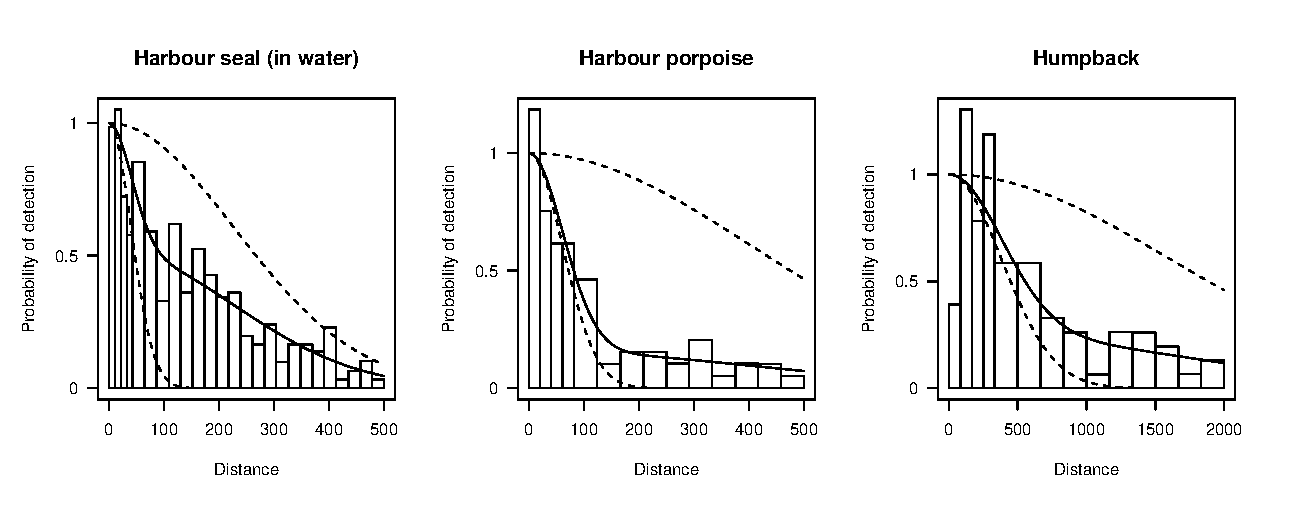
\includegraphics[width=\textwidth]{analyses/williamsplots.eps}
\caption{Plots of the detection functions fit to the Williams and Thomas (2007) data.}
\label{williams-detfcts}
\end{figure}



\subsection{Wood ants in the Abernethy forest}
line transects w. covars + spikes

[[TKTKTK ants paper cite]] analyse data on two species of wood ant (\textit{Formica aquilonia} and \textit{Formica lugubris}) in the Abernethy Forest in Strathspey Scotland over the period of August--September 2003. The number of nests sighted was 150 out to a distance of 72.04m from the track line, although 45\% of the nest sightings lay within 4m of the line. As part of their analysis several different truncation distances were used and larger truncation distances led to large variance in the encounter rate estimates and hence in overall abundance estimates[[TKTKTK ants paper cite]]. This is due to the spike caused by the large number of detections close to the line.

[[TKTKTK probably want to use the same binning here as in the paper]]

\subsection{Long-finned pilot whales}
line transects w. covars

\subsection{Amakihi}
point transects w. covars

[[Big results table here comparing the results from the relevant papers and what we got]]




\section{Discussion}
\label{s:discuss}

Package on CRAN

Has usual methods

Will be in next version of Distance?!



%  The \backmatter command formats the subsequent headings so that they
%  are in the journal style.  Please keep this command in your document
%  in this position, right after the final section of the main part of 
%  the paper and right before the Acknowledgements, Supplementary Materials,
%  and References sections. 

\backmatter

%  This section is optional.  Here is where you will want to cite
%  grants, people who helped with the paper, etc.  But keep it short!

\section*{Acknowledgements}

David would like to acknowledge the (financial) support of EPSRC.

Both authors would like to thank David Borchers, who suggested the parametrisation for the mixture proportions.


\section{Appendix A - Derivatives}

\subsection{Line transects}

Starting from the likelihood given in (\ref{lt-lik}), we derive the derivatives with respect to the optimisation parameters.

\subsection{With respect to $\beta_{0j*}$}
For the intercept terms (also considering in the non-covariate case, these are just the parameters), the parameters have no effect outside of their mixture (ie. $\beta_{0j*}$ only has an influence on mixture component $j*$), so we can write:
\begin{equation}
\frac{\partial l(\bm{\theta},\bm{\phi}; \mathbf{x},\mathbf{Z})}{\partial \beta_{0j*}} = \sum_{i=1}^n \frac{1}{g(x_i,\mathbf{Z}; \bm{\theta},\bm{\phi})} \phi_{j*} \frac{\partial}{\partial \beta_{0j*}} g_{j*}(x_i,\mathbf{Z}; \bm{\theta}_{j*})  - \frac{\phi_{j*}}{\mu_i}  \frac{\partial}{\partial \beta_{0j*}} \mu_{ij*}.
\end{equation}
Now, to first fine $\frac{\partial}{\partial \beta_{0j*}} g_{j*}(x_i,\mathbf{Z}; \bm{\theta}_{j*})$:
\begin{equation*}
\frac{\partial g_{j*}(x_i,\mathbf{Z}; \bm{\theta}_{j*})}{\partial \beta_{0j*}} = \frac{\partial}{\partial \beta_{0j*}} \exp\Big( -\frac{x_i^2}{2\sigma_{j*}^2} \Big)
\end{equation*}
applying the chain rule and remembering that $\sigma_{j*}$ is a (trivial) function of the $\beta_{0j}$s:
\begin{equation*}
\frac{\partial g_{j*}(x_i,\mathbf{Z}; \bm{\theta}_{j*})}{\partial \beta_{0j*}} = \Big( \frac{x_i}{\sigma_{j*}}\Big)^2 \exp \Big(-\frac{x_i^2}{2 \sigma_{j*}^2}\Big)
\end{equation*}

Expressing $\mu_{ij*}$ in terms of the error function:
\begin{align}
\frac{\partial \mu_{ij*}}{\partial \beta_{0j*}} &= \frac{\partial}{\partial \beta_{0j*}} \Big( \sqrt{\frac{\pi}{2}} \sigma_{j*} \text{Erf}\Big(\frac{w}{\sqrt{2\sigma_{j*}^2}}\Big) \Big)\\
&= \text{Erf}\Big(\frac{w}{\sqrt{2\sigma_{j*}^2}}\Big) \frac{\partial}{\partial \beta_{0j*}} \Big( \sqrt{\frac{\pi}{2}} \sigma_{j*} \Big) + \sqrt{\frac{\pi}{2}} \sigma_{j*} \frac{\partial}{\partial \beta_{0j*}} \Big(\text{Erf}\Big(\frac{w}{\sqrt{2\sigma_{j*}^2}}\Big) \Big)
\label{app-mu-erf}
\end{align}
To find $\frac{\partial}{\partial \beta_{0j*}} \text{Erf}\Big(\frac{w}{\sqrt{2\sigma_{j*}^2}}\Big)$, note that we can write and then apply the chain rule:
\begin{align*}
\frac{\partial}{\partial \beta_{0j*}} \text{Erf}\Big(\frac{w}{\sqrt{2\sigma_{j*}^2}}\Big) &= \frac{\partial}{\partial \beta_{0j*}} S(u(\sigma_{j*}))\\
&= \frac{\partial S(u)}{\partial u} \frac{\partial u(\sigma_{j*})}{\partial \sigma_{j*} } \frac{\partial \sigma_{j*}}{\partial \beta_{0j*}}
\end{align*}
where 
\begin{align*}
S(u) = \int_0^{u} \exp(-t^2) \text{d}t \quad \text{and} \quad u(\sigma_{j*})=\frac{w}{\sqrt{2\sigma_{j*}^2}}.
\end{align*}
Their derivatives being
\begin{align*}
\frac{\partial S(u)}{\partial u} = \frac{2}{\sqrt{\pi}} \exp(-u^2) \text{,} \quad \frac{\partial u(\sigma_{j*})}{\partial \sigma_{j*}} = -\frac{w}{\sqrt{2}}\sigma_{j*}^{-2}.
\end{align*}
Given these terms, it's just a case of multiplying them:
\begin{align*}
\frac{\partial S(u)}{\partial u} \frac{\partial u(\sigma_{j*})}{\partial \sigma_{j*} } \frac{\partial \sigma_{j*}}{\partial \beta_{0j*}} = - \sqrt{\frac{2}{\pi}} \frac{w}{\sigma_{j*}} \exp\Big( -\frac{w^2}{2\sigma_{j*}^2} \Big)
\end{align*}
Substituting into (\ref{app-mu-erf}):
\begin{equation*}
\frac{\partial \mu_{ij*}}{\partial \beta_{0j*}} =  \mu_{ij*} - w \exp\Big( -\frac{w^2}{2\sigma_{j*}^2} \Big)
\end{equation*}
Finally, the derivative is:
\begin{equation}
\frac{\partial l(\bm{\theta}, \bm{\phi}; \mathbf{x},\mathbf{Z})}{\partial \beta_{0j*}} = \sum_{i=1}^n \Big( \frac{x_i}{\sigma_{j*}}\Big)^2 \phi_{j*} \frac{g_{j*}(x_i,\mathbf{Z}; \bm{\theta}_{j*})}{g(x_i,\mathbf{Z}; \bm{\theta},\bm{\phi})}  - \frac{\phi_{j*}}{\mu_i} (\mu_{ij*} - w g_{j*}(w,\mathbf{Z}; \bm{\theta}_{j*})).
\end{equation}



\subsection{With respect to $\beta_{k*}$}

Derivatives with respect to the common covariate parameters are found in a similar way to above. The expressions are slightly more complicated since the $\beta_k$s effect all of the mixture components.
\begin{equation}
\frac{\partial l(\bm{\theta},\bm{\phi}; \mathbf{x},\mathbf{Z})}{\partial \beta_{k*}} = \sum_{i=1}^n \Big( \frac{1}{g(x_i,\mathbf{Z}; \bm{\theta},\bm{\phi})} \sum_{j=1}^J \phi_j \frac{\partial}{\partial \beta_{k*}} g_j(x_i,\mathbf{Z}; \bm{\theta}_j) - \frac{1}{\mu_i} \sum_{j=1}^J \phi_j \frac{\partial}{\partial \beta_{k*}}\mu_{ij}\Big)
\end{equation}
Every $\sigma_{j}$ is a function of the $\beta_{k}$s, so:
\begin{align*}
\frac{\partial \sigma_{j}}{\partial \beta_{k*}} &= \frac{\partial}{\partial \beta_{0j*}} \exp \Big( \beta_{0j} + \sum_{k=1}^K z_{ik} \beta_{k}\Big),\\
&= z_{ik*} \exp \Big( \beta_{0j} + \sum_{k=1}^K z_{ik} \beta_{k}\Big),\\
&= z_{ik*}\sigma_{j}.
\end{align*}
Hence:
\begin{equation*}
 \frac{\partial}{\partial \beta_{k*}} \exp\Big( -\frac{x^2}{2\sigma_{j}^2} \Big) = z_{k*} \Big( \frac{x}{\sigma_{j}}\Big)^2 \exp \Big(-\frac{x^2}{2 \sigma_{j}^2}\Big) 
\end{equation*}
And so for the $\mu_{ij}$s:
\begin{equation*}
\frac{\partial \mu_{ij}}{\partial \beta_{k*}} = z_{ik*} \Big( \mu_{ij} - w \exp\Big( -\frac{w^2}{2\sigma_{j}^2} \Big) \Big)
\end{equation*}
The derivative is then:
\begin{equation*}
\frac{\partial l(\bm{\theta},\bm{\phi}; \mathbf{x},\mathbf{Z})}{\partial \beta_{k*}} = \sum_{i=1}^n \Big( \frac{1}{g(x_i,\mathbf{Z}; \bm{\theta},\bm{\phi})} \sum_{j=1}^J \phi_j  z_{k*} \Big( \frac{x_i}{\sigma_{j}}\Big)^2 g_j(x_i,\mathbf{Z}; \bm{\theta}_j) - \frac{1}{\mu_i} \sum_{j=1}^J \phi_j z_{ik*} ( \mu_{ij} - w g_j(x_i,\mathbf{Z}; \bm{\theta}_j) )\Big)
\end{equation*}



\subsubsection{With respect to $\alpha_{j*}$}

First note that we can write the likelihood (\ref{lt-lik}) as:
\begin{align*}
l(\bm{\theta},\bm{\phi}; \mathbf{x},\mathbf{Z}) = \sum_{i=1}^n\Big( &\log \Big( \sum_{j=1}^{J-1} \phi_j g_j(x_i,\mathbf{Z}; \bm{\theta}_j) + (1-\sum_{j=1}^{J-1} \phi_j) g_J(x_i,\mathbf{Z}; \bm{\theta}_J)\Big) \\
&-  \log \Big(\sum_{j=1}^{J-1} \phi_j \mu_{ij} + (1-\sum_{j=1}^{J-1} \phi_j) \mu_{ij} \Big) \Big)
\end{align*}
The derivatives with respect to the $\alpha_{j*}$ of this expression are then:
\begin{align}
\frac{\partial l(\bm{\theta},\bm{\phi}; \mathbf{x},\mathbf{Z})}{\partial \alpha_{j*}} = &\Big( \sum_{i=1}^n \frac{1}{g(x_i,\mathbf{Z}; \bm{\theta},\bm{\phi})} \Big( \sum_{j=1}^{J-1} g_j(x_i,\mathbf{Z}; \bm{\theta}_j) \frac{\partial \phi_j}{\partial \alpha_{j*}}  -g_J(x_i,\mathbf{Z}; \bm{\theta}_J) \sum_{j=1}^{J-1}  \frac{\partial \phi_j}{\partial \alpha_{j*}}\Big) \\
&- \frac{1}{\mu_i} \Big(\sum_{j=1}^{J-1} \mu_{ij} \frac{\partial \phi_j}{\partial \alpha_{j*}} - \mu_{iJ} \sum_{j=1}^{J-1}   \frac{\partial \phi_j}{\partial \alpha_{j*}} \Big)\Big)
\label{app-lik-alphad}
\end{align}
Finding the derivatives is then simply a matter of finding the derivatives of $\phi_{j}$ with respect to $\alpha_{j*}$ and substituting them back into (\ref{app-lik-alphad}).
\begin{equation*}
\frac{\partial \phi_j}{\partial \alpha_{j*}} = \frac{\partial}{\partial \alpha_{j*}}F(\sum_{p=1}^j e^{\alpha_p}) - \frac{\partial}{\partial \alpha_{j*}} F(\sum_{p=1}^{j-1} e^{\alpha_p}).
\end{equation*}
Looking at each of the terms:
\begin{equation*}
\frac{\partial}{\partial \alpha_{j*}} F(\sum_{p=1}^j e^{\alpha_p})=A_{j}=\begin{cases}
e^{\alpha_{j*}}f(\sum_{p=1}^j e^{\alpha_p})& \text{for $j\geq j*$},\\
0 & \text{for $j<j*$}.
\end{cases}
\end{equation*}
and
\begin{equation*}
\frac{\partial}{\partial \alpha_{j*}} F(\sum_{p=1}^{j-1} e^{\alpha_p})=A_{(j-1)}=\begin{cases}
e^{\alpha_{j*}}f(\sum_{p=1}^{j-1} e^{\alpha_p})& \text{for $j-1\geq j*$},\\
0 & \text{for $j-1<j*$}.
\end{cases}
\end{equation*}
So
\begin{equation*}
\frac{\partial \phi_j}{\partial \alpha_{j*}} = A_j - A_{j-1}.
\end{equation*}
Substituting these back into (\ref{app-lik-alphad}) and re-arranging gives:
\begin{align*}
\frac{\partial l(\bm{\theta},\bm{\phi}; \mathbf{x},\mathbf{Z})}{\partial \alpha_{j*}} = \sum_{i=1}^n & \Big( \frac{1}{g(x_i,\mathbf{Z}; \bm{\theta},\bm{\phi})} \sum_{j=1}^{J-1} (A_j - A_{j-1}) (g_j(x,\mathbf{Z}; \bm{\theta}_j) - g_J(x,\mathbf{Z}; \bm{\theta}_J))\\
&- \frac{1}{\mu_i} \sum_{j=1}^{J-1}(A_j - A_{j-1})(\mu_{ij} - \mu_{iJ}) \Big)
\end{align*}


\subsection{Point transects}

\subsubsection{With respect to $\beta_{0j}$}

Starting with the likelihood in (\ref{pt-lik}), one can see that we obtain:
\begin{align*}
\frac{\partial l(\bm{\theta}, \bm{\phi}; \mathbf{r},\mathbf{Z})}{\partial \beta_{0j*}}  &= \sum_{i=1}^n \Big( \frac{\partial}{\partial \beta_{0j*}} \log \sum_{j=1}^J \phi_j g_j(r_i,\mathbf{Z}; \bm{\theta}_j) - \frac{\partial}{\partial \beta_{0j*}}\log \sum_{j=1}^J \phi_j \nu_{ij}\Big)\\
&= \sum_{i=1}^n \Big( \frac{ \phi_{j*} \frac{\partial}{\partial \beta_{0j*}}  g_{j*} (r_i,\mathbf{Z}; \bm{\theta}_j)}{g(r_i,\mathbf{Z}; \bm{\theta}, \bm{\phi})} - \frac{ \phi_{j*}\frac{\partial}{\partial \beta_{0j*}}  \nu_{ij*} }{ \sum_{j=1}^J \phi_j \nu_{ij}}\Big)
\end{align*}
the first part of which (the derivatives of the detection function) are as in the line transect case. The derivatives of $\nu_{ij}$ are simpler in the point transect case, since there is an easy analytic expression for $\nu_{ij}$ when $g_j$ is half-normal :
\begin{equation*}
\nu_{ij} = 2 \pi \sigma_{ij} (1-\exp (-w^2/2\sigma_{ij} )
\end{equation*}
then simply applying the product rule yields:
\begin{equation*}
\frac{\partial \nu_{ij}}{\partial \beta_{0j*}} = 2 \pi (2 \sigma_{ij*} + g_{j*}(w) \Big(\frac{w^2}{\sigma_{ij*}} - 2\sigma_{ij*}\Big)).
\end{equation*}
Substituting this into the above expression:
\begin{equation*}
\frac{\partial l(\bm{\theta}, \bm{\phi}; \mathbf{r},\mathbf{Z})}{\partial \beta_{0j*}}  = \sum_{i=1}^n \Big( \frac{ \phi_{j*} (r_i/\sigma_{j*})^2 g_{j*}(r_i,\mathbf{Z}; \bm{\theta}_{j*})}{g(r_i,\mathbf{Z}; \bm{\theta}, \bm{\phi})} - \frac{ \phi_{j*} 2 \pi (2 \sigma_{ij} + g_{j*}(w,\mathbf{Z}; \bm{\theta}_{j*}) (w^2/\sigma_{ij*} - 2\sigma_{ij*})) }{ \sum_{j=1}^J \phi_j \nu_{ij}}\Big)
\end{equation*}

\subsection{With respect to $\beta_{k*}$}

TKTKTK

\begin{align*}
\frac{\partial l(\bm{\theta}, \bm{\phi}; \mathbf{r},\mathbf{Z})}{\partial \beta_{0j*}}  &= \sum_{i=1}^n \Big( \frac{\partial}{\partial \beta_{0j*}} \log \sum_{j=1}^J \phi_j g_j(r_i,\mathbf{Z}; \bm{\theta}_j) - \frac{\partial}{\partial \beta_{0j*}}\log \sum_{j=1}^J \phi_j \nu_{ij}\Big)\\
&= \sum_{i=1}^n \Big( \frac{ \sum_{j=1}^J \phi_{j} \frac{\partial}{\partial \beta_{0j*}}  g_{j} (r_i,\mathbf{Z}; \bm{\theta}_j)}{g(r_i,\mathbf{Z}; \bm{\theta}, \bm{\phi})} - \frac{ \sum_{j=1}^J \phi_{j}\frac{\partial}{\partial \beta_{0j*}}  \nu_{ij} }{ \sum_{j=1}^J \phi_j \nu_{ij}}\Big)
\end{align*}


\section{Appendix B - rejection sampling for simulation of mixture detection function distance data}

We generate $n$ samples by sampling distances $X\sim \text{Uniform}(0,w)$ distribution. We want $X$ to come from the PDF of the distances, $f$. We know that in the line transect case that the maximum value of $f$ is $1/\mu$ (since $\mu=1/f(0)$ and f(0) is the maximum of $f$). So we can then set
\begin{equation}
M \geq \frac{1}{\mu},
\end{equation}
so finding $h(x)$,
\begin{align*}
h(x) &= \frac{f(x)}{U(x) M}\\
&= \frac{g(x)/\mu}{(1/w) (1/\mu)}\\
&= \frac{\sum_{j=1}^J \phi_j g_j(x)/\mu}{(1/w) (1/\mu)}\\
&= w \sum_{j=1}^J \phi_j g_j(x)
\end{align*}

then, generating a $U \sim \text{Uniform}(0,1)$ accept $X$ if 
\begin{equation}
U \leq wg(X,z_i; \bm{\theta}, \bm{\phi}).
\end{equation}
where $z_i$ indicates the covariates that are to be used for generated observation $i$.

MORE HERE

%  Here, we create the bibliographic entries manually, following the
%  journal style.  If you use this method or use natbib, PLEASE PAY
%  CAREFUL ATTENTION TO THE BIBLIOGRAPHIC STYLE IN A RECENT ISSUE OF
%  THE JOURNAL AND FOLLOW IT!  Failure to follow stylistic conventions
%  just lengthens the time spend copyediting your paper and hence its
%  position in the publication queue should it be accepted.

%  We greatly prefer that you incorporate the references for your
%  article into the body of the article as we have done here 
%  (you can use natbib or not as you choose) than use BiBTeX,
%  so that your article is self-contained in one file.
%  If you do use BiBTeX, please use the .bst file that comes with 
%  the distribution.


Bibiolography - TKTKTK

Buckland et al 2001

Buckland 1992

ants paper

Pledger

Dorazio and Royle

Morgan and Ridout


\begin{thebibliography}{}

\bibitem{ }  Buckland, S. T., Anderson, D. R., Burnham, K. P., Laake, J. L., Borchers, D. L., and Thomas, L.  (2004). \textit{Advanced Distance Sampling}. Oxford University Press. Oxford, UK.

\bibitem{ } Marques, T. A., Thomas, L., Fancy, S. G., Buckland, S. T. (2007). Improving estimates of bird density using multiple-covariate distance sampling. \textit{The Auk} \textbf{124}(9), pp. 1229--1243.

\bibitem{ } Williams, R. and Thomas, L. (2007). Distribution and abundance of marine mammals in the coastal waters of British Columbia, Canada. \textit{Journal of Cetacean Research and Management} \textbf{9}(1), pp. 15--38.

\bibitem{ } Pike, D. G., Gunnlaugsson, T., V\'{i}kingsson, G .A., Desportes, G. and Mikkelson, B.  (2003) An estimate of the abundance of long-finned pilot whales (\textit{globicephala melas}) from the NASS-2001 shipboard survey. Paper SC/11/AE/10 presented to the North Atlantic Marine Mammal Commission (NAMMCO) Scientific Committee Working Group on Abundance Estimates.





\end{thebibliography}


\label{lastpage}

\end{document}

